\documentclass[border=2pt,tikz]{standalone}
\usepackage{tikz}
\usetikzlibrary{calc}
\begin{document}
	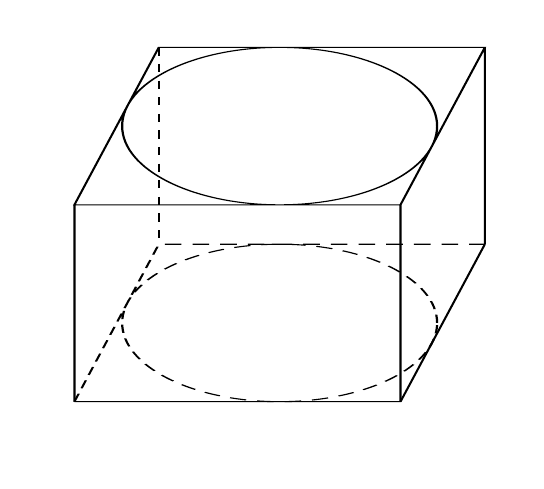
\begin{tikzpicture}
		\clip (-3.2,-1.75) rectangle (3,3.75);
		\draw[transform canvas={cm={2,0,0,1,(0,0)}},densely dashed]
		(-1,-1) coordinate (At) (1,-1) coordinate (Bt)
		(-1,1) coordinate (Ct) (1,1) coordinate (Dt)
		(0,0) circle (1)
		(-15:1) coordinate (Tm)
		([rotate around={90:(Tm)}]0,0) coordinate (Ap)
		(intersection of Ap--Tm and At--Bt) coordinate (B)
		(intersection of Ap--Tm and Ct--Dt) coordinate (C)
		(165:1) coordinate (Th)
		([rotate around={90:(Th)}]0,0) coordinate (Ap)
		(intersection of Ap--Th and At--Bt) coordinate (A)
		(intersection of Ap--Th and Ct--Dt) coordinate (D)
		(A)--(D)--(C);
		\draw[transform canvas={cm={2,0,0,1,(0,0)}}]
		(A)--(B)--(C);
		
		\draw[transform canvas={cm={2,0,0,1,(0,2.5)}}]
		(-1,-1) coordinate (At) (1,-1) coordinate (Bt)
		(-1,1) coordinate (Ct) (1,1) coordinate (Dt)
		(0,0) circle (1)
		(-15:1) coordinate (Tm)
		([rotate around={90:(Tm)}]0,0) coordinate (Ap)
		(intersection of Ap--Tm and At--Bt) coordinate (B')
		(intersection of Ap--Tm and Ct--Dt) coordinate (C')
		(165:1) coordinate (Th)
		([rotate around={90:(Th)}]0,0) coordinate (Ap)
		(intersection of Ap--Th and At--Bt) coordinate (A')
		(intersection of Ap--Th and Ct--Dt) coordinate (D')
		(C')--(B')--(A')--(D')--cycle
		\foreach \x in {B',A',C'}{
			(\x)--+(0,-2.5)};
		\draw[transform canvas={cm={2,0,0,1,(0,2.5)}},dashed]
		(D')--+(0,-2.5);
	\end{tikzpicture}
\end{document} 